\documentclass[12pt,en,a4paper]{article}
\usepackage{vntex}
\usepackage[utf8]{inputenc}
\usepackage{amsmath, anyfontsize, caption, color, enumerate, fancyhdr, float, graphicx, lastpage, listings, natbib, pifont, tikz}
\usepackage[open,openlevel=1]{bookmark}
\usepackage[framemethod=tikz]{mdframed}
\usetikzlibrary{calc,backgrounds}
\newcommand\HRule{\rule{12cm}{1pt}}
\pagestyle{fancy}
\fancyhead{} % clear all header fields
\fancyhead[L]{
	\color{blue}
	\begin{tabular}{rl}
		\begin{picture}(25,15)(0,0)
		\put(0,-8){
\includegraphics[width=8mm, height=8mm]{BK.png}}
		\end{picture}
		\begin{tabular}{l}
			\textbf{\bf \ttfamily Ho Chi Minh University of Technology}\\
			\textbf{\bf \ttfamily Faculty of Computer Science \& Engineering}
		\end{tabular} 	
	\end{tabular}
}
\fancyhead[R]{
	\begin{tabular}{l}
		\tiny \bf \\
		\tiny \bf 
	\end{tabular}
}
\fancyfoot{} % clear all footer fields
\fancyfoot[L]{\scriptsize \ttfamily Linear Algebra Assignment}
\fancyfoot[R]{\scriptsize \ttfamily Page {\thepage}/\pageref{LastPage}}
\renewcommand{\headrulewidth}{0.3pt}
\renewcommand{\footrulewidth}{0.3pt}

\definecolor{dkgreen}{rgb}{0,0.6,0}
\definecolor{gray}{rgb}{0.5,0.5,0.5}
\definecolor{mauve}{rgb}{0.58,0,0.82}

\lstset{frame=tb,
	language=Matlab,
	aboveskip=3mm,
	belowskip=3mm,
	showstringspaces=false,
	columns=flexible,
	basicstyle={\small\ttfamily},
	numbers=none,
	numberstyle=\tiny\color{gray},
	keywordstyle=\color{blue},
	commentstyle=\color{dkgreen},
	stringstyle=\color{mauve},
	breaklines=true,
	breakatwhitespace=true,
	tabsize=3,
	numbers=left,
	stepnumber=1,
	numbersep=1pt,    
	firstnumber=1,
	numberfirstline=true
}

\begin{document}
	\begin{titlepage}
		
\begin{tikzpicture}[remember picture, overlay]
		\draw[line width = 2pt] ($(current page.north west) + (1in,-1in)$) rectangle ($(current page.south east) + (-1in,1in)$);
		\end{tikzpicture}
		
		\begin{center}
			% Upper part of the page
			\textbf{\fontsize{12pt}{1pt}\selectfont HO CHI MINH CITY UNIVERSITY OF TECHNOLOGY}\\[0.5cm]
			{\fontsize{13pt}{1pt}\selectfont Faculty of Computer Science \& Engineering}\\[0.5cm]
			\begin{figure}[h]
				\centering
				
\includegraphics[width=1.7in,height=1.7in]{BK.png}
			\end{figure}
			
			% Title
			\HRule \\[0.5cm]
			{ \textbf{\fontsize{20pt}{1pt}\selectfont LINEAR ALGEBRA ASSIGNMENT}}\\[0.4cm]
			
			\HRule \\[0.8cm]
			\begin{minipage}{0.545\textwidth}   
				\begin{flushleft} 
					\textbf{Authors:}\\
					\begin{tabular}{l l}
						Nguyễn Hoàng & 1952255 \\
						Tạ Minh Huy & 1952268 \\
						Ho Trí Kháng & 1952069 \\
						Nguyễn Đình Khương Duy & 1952207 \\
					\end{tabular}
				\end{flushleft}
			\end{minipage}
			\begin{minipage}{0.4\textwidth}
				\begin{flushright} 
					\textbf{Class:}\\
					MT1008\\
					\textbf{Lecturer:}\\
					Hoàng Hải Hà\\
					
				\end{flushright}
			\end{minipage}
			
			\vfill
			
			% Bottom of the page
			\vspace{2cm}
			{\large} %{\large \today}
		\end{center}
	\end{titlepage}
	
	\pdfbookmark[0]{Problem 1}{prob1}
	\section*{Problem 1}
	\pdfbookmark[1]{a:}{prob1a}
	\subsection*{a)}
	The following code provides the required matrix
	\begin{mdframed}[hidealllines=true,backgroundcolor=magenta!10]
		\begin{lstlisting}
		>> A = [1/3 1/4 0 1/4 0 0 0 0 0;
		1/3 1/4 1/3 0 1/5 0 0 0 0;
		0 1/4 1/3 0 0 1/4 0 0 0;
		1/3 0 0 1/4 1/5 0 1/3 0 0;
		0 1/4 0 1/4 1/5 1/4 0 1/4 0;
		0 0 1/3 0 1/5 1/4 0 0 1/3;
		0 0 0 1/4 0 0 1/3 1/4 0;
		0 0 0 0 1/5 0 1/3 1/4 1/3;
		0 0 0 0 0 1/4 0 1/4 1/3]
		\end{lstlisting}
	\end{mdframed}
	And we receive
	\begin{figure}[H]
		\centering
		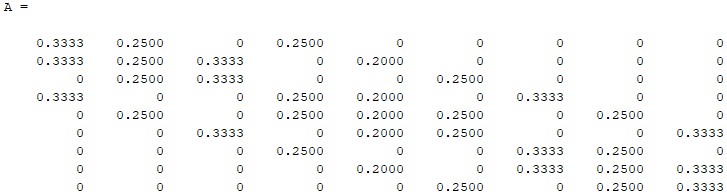
\includegraphics[scale=0.7]{prob1a.png}
		\label{prob1a}
	\end{figure}
	\pdfbookmark[1]{b:}{prob1b}
	\subsection*{b)}
	We construct a 9 $\times$ 1 matrix for the initial state (room 4 is 1, other rooms are 0):
	\begin{mdframed}[hidealllines=true,backgroundcolor=magenta!10]
		\begin{lstlisting}
		>> X0 = [0; 0; 0; 1; 0; 0; 0; 0; 0]
		\end{lstlisting}
	\end{mdframed}
	\[
	\begin{tabular}{l r}
	X0 = & \\
	& 0 \\
	& 0 \\
	& 0 \\
	& 1 \\
	& 0 \\
	& 0 \\
	& 0 \\
	& 0 \\
	& 0 
	\end{tabular}
	\]
	The state after 5 step, using the formula: \(X5 = A^5 \cdot X0\)
	\begin{mdframed}[hidealllines=true,backgroundcolor=magenta!10]
		\begin{lstlisting}
		>> X5 = A^5 * X0
		\end{lstlisting}
	\end{mdframed}
	\[
	\begin{tabular}{l r}
	X5 = & \\
	& 0.1186 \\
	& 0.1182 \\
	& 0.0667 \\
	& 0.1569 \\
	& 0.1558 \\
	& 0.0804 \\
	& 0.1186 \\
	& 0.1182 \\
	& 0.0667
	\end{tabular}
	\]
	As we can see, \(X5(9,1)=0.0667\), so the probability is $0.0667$.
	\pdfbookmark[1]{c:}{prob1c}
	\subsection*{c)}
	We use the following command to find eigenvalue and eigenvector:
	\begin{mdframed}[hidealllines=true,backgroundcolor=magenta!10]
		\begin{lstlisting}
		>> [S D] = eig(A)
		\end{lstlisting}
	\end{mdframed}
	\begin{figure}[H]
		\centering
		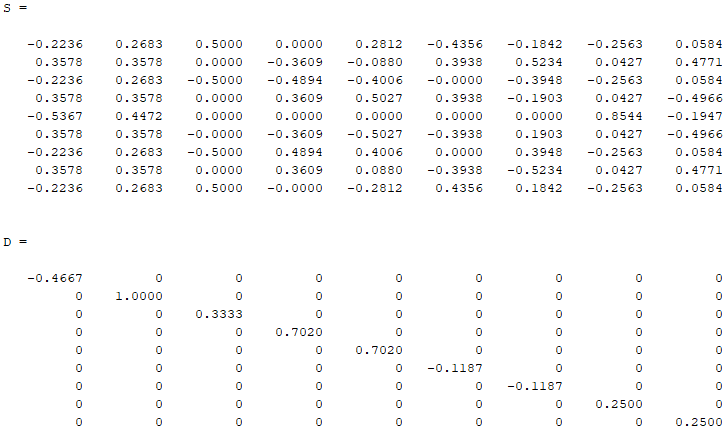
\includegraphics[scale=0.7]{prob1c.png}
		\label{prob1c}
	\end{figure}
	The eigenvalue lamda corresponding to the steady state is 1. So take the column of $S$ corresponding to the column that contains $1$ in $D$. \\
	To extract that column, we get the steady state
	\begin{mdframed}[hidealllines=true,backgroundcolor=magenta!10]
		\begin{lstlisting}
		>> Stead = [S(:,2)]
		\end{lstlisting}
	\end{mdframed}
	\begin{figure}[H]
		\centering
		\includegraphics*[scale=0.8]{prob1c1.png}
		\label{prob1c1}
	\end{figure}
	\newpage
	\pdfbookmark[0]{Problem 2}{prob2}
	\section*{Problem 2}
	\begin{figure}[H]
		\centering
		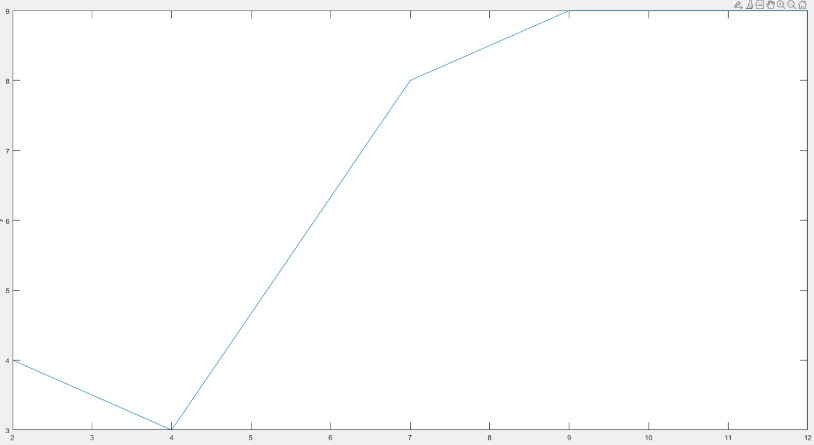
\includegraphics[scale=0.7]{prob2.png}
		\label{prob2}
	\end{figure}
	
	\newpage
	\pdfbookmark[0]{Problem 3}{prob3}
	\section*{Problem 3}
	First, we enter the encoding matrix.
	\begin{mdframed}[hidealllines=true,backgroundcolor=magenta!10]
		\begin{lstlisting}
		>> A = [1 2 3; 1 1 2; 0 1 2];
		\end{lstlisting}
	\end{mdframed}
	\pdfbookmark[1]{a:}{prob3a}
	\subsection*{a)}
	The message SEND HIM MONEY can be express in matrix as:
	\begin{mdframed}[hidealllines=true,backgroundcolor=magenta!10]
		\begin{lstlisting}
		>> B = [19 5 14; 4 0 8; 9 13 0; 13 15 14; 5 25 0];
		\end{lstlisting}
	\end{mdframed}
	We encode the message by multiplying $B$ with $A$.
	\begin{mdframed}[hidealllines=true,backgroundcolor=magenta!10]
		\begin{lstlisting}
		>> B * A;
		\end{lstlisting}
	\end{mdframed}
	And we get the result \\
	\[
	\begin{tabular}{l r r r}
	ans & = & & \\
	& 24 & 57 & 95 \\
	& 4 & 16 & 28 \\
	& 22 & 31 & 53 \\
	& 28 & 55 & 97 \\
	& 30 & 35 & 65
	\end{tabular}
	\]
	\pdfbookmark[1]{b:}{pro3b}
	\subsection*{b)}
	The following instruction enters the encoded message:
	\begin{mdframed}[hidealllines=true,backgroundcolor=magenta!10]
		\begin{lstlisting}
		>> B = [67 44 41; 49 39 19; 113 76 62; 104 69 55];
		\end{lstlisting}
	\end{mdframed}
	To decode the message, we multiply $B$ with the inverse of $A$.
	\begin{mdframed}[hidealllines=true,backgroundcolor=magenta!10]
		\begin{lstlisting}
		>> B * inv(A)
		\end{lstlisting}
	\end{mdframed}
	The decoded message is \\
	\[
	\begin{tabular}{l r r r}
	ans & = & & \\
	& 47 & 20 & -70 \\
	& 59 & -10 & -69 \\
	& 90 & 23 & -127 \\
	& 83 & 21 & -118
	\end{tabular}
	\]
	\newpage
	\pdfbookmark[0]{Problem 4}{prob4}
	\section*{Problem 4}
	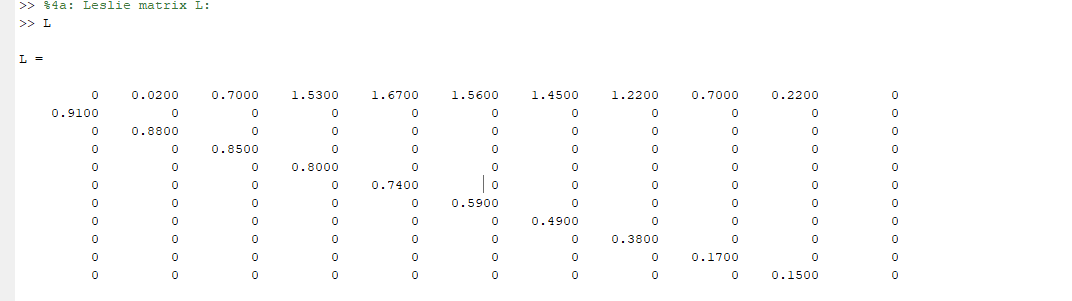
\includegraphics[scale = .7]{prob4aLeslie.png}
	\begin{mdframed}[hidealllines=true,backgroundcolor=magenta!10]
		\begin{lstlisting}
		>> [S D] = eig(L)
		\end{lstlisting}
	\end{mdframed}
	\begin{figure}[H]
		\centering
		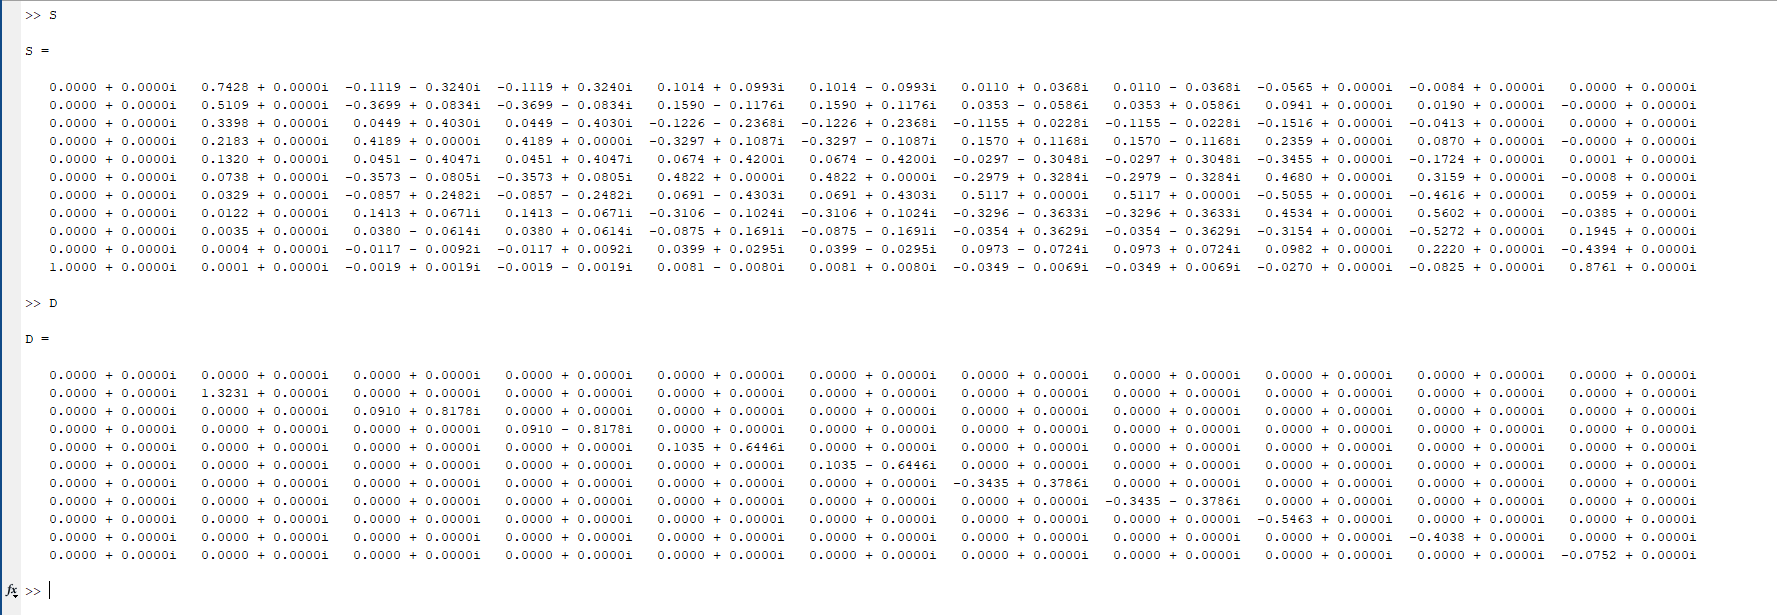
\includegraphics[scale = .4]{prob4aEigen.png}
		\label{prob4aE}
		\caption*{Eigen value and Eigen vector}
	\end{figure}
	There is only one positive eigenvalue(column 2 of the matrix D, as above). The corresponding eigenvector is column vector 2 of the matrix S(as above).\\
	\pdfbookmark[1]{b:}{prob4b}
	\subsection*{b)}
	\begin{figure}[H]
		\centering
		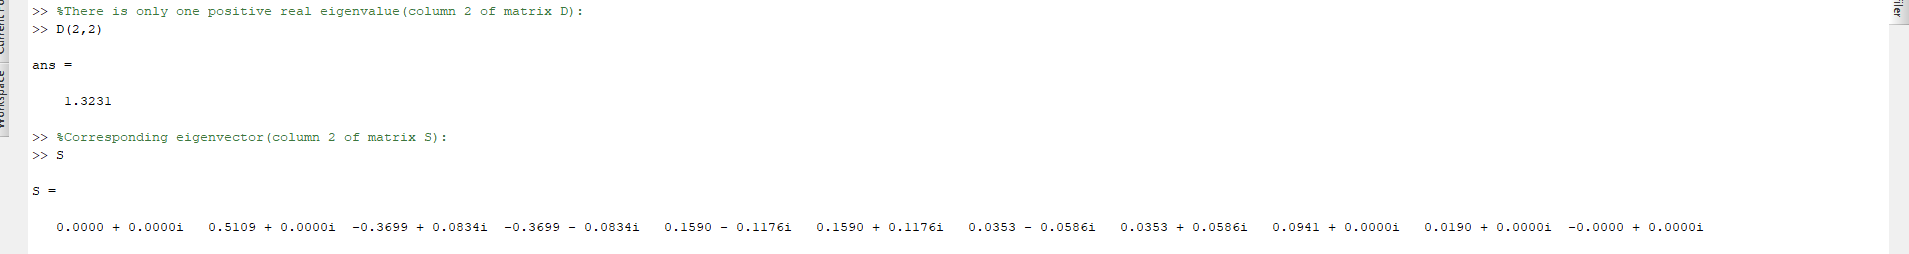
\includegraphics[scale = .4]{prob4aEigenVal.png}
		\label{prob4aEV}
		\caption*{Eigen value and Eigen vector}
	\end{figure}
	\begin{figure}
		\centering
		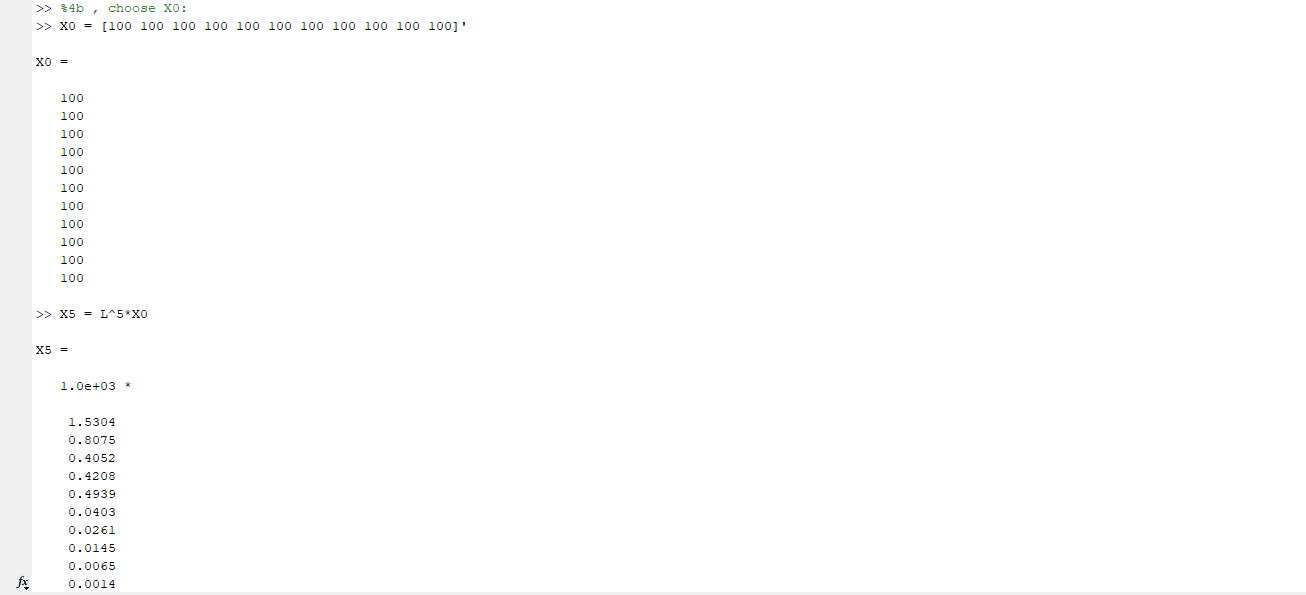
\includegraphics[scale = .7]{prob4bX5.png}
		\label{prob4bX5}
		\caption*{Initial state and number of seals after 5 years}
	\end{figure}
	\begin{figure}
		\centering
		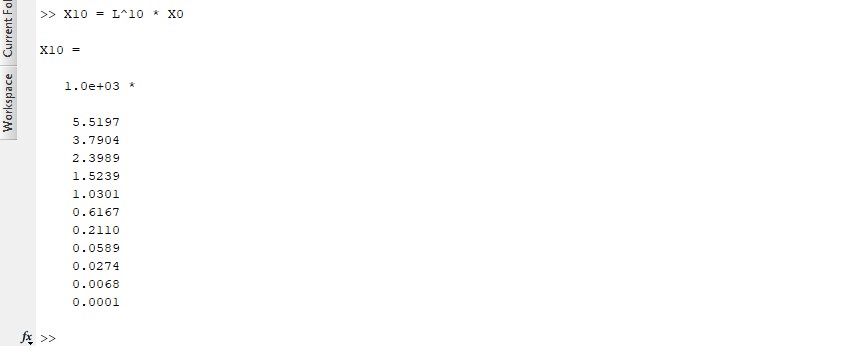
\includegraphics[scale = .7]{prob4bX10.png}
		\label{prob4bX10}
		\caption*{Number of seals after 10 years}
	\end{figure}
	\newpage
	\pdfbookmark[0]{Problem 5}{prob5}
	\section*{Problem 5}
	\subsection*{a)}
	The coefficient of the matrix from subspace $F$ can be expressed as
	\begin{figure}[H]
		\centering
		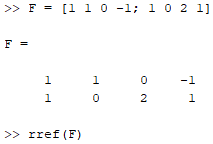
\includegraphics[scale=0.8]{prob5a1.png}
		\label{prob5c1}
	\end{figure}
	The result can be obtained by reducing the given matrix to echelon form
	\begin{figure}[H]
		\centering
		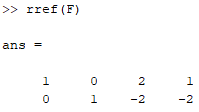
\includegraphics[scale=0.8]{prob5a2.png}
		\label{prob5a2}
	\end{figure}
	The basis is $\{(1,0,2,1),(0,1,-2,-2)\}$
	\subsection*{b)}
	The projection of vector $x=(2, 5, 8, 9)$ on F can be expressed as
	\begin{equation*}
	y=proj_{F}x = \lambda_1 e_1 + \lambda_2 e_2
	\end{equation*}
	$\Rightarrow$ \(\langle x, e_1 \rangle = \lambda_1 \langle e_1, e_1\rangle + \lambda_2 \langle e_1, e_1 \rangle\), \(\langle x, e_2 \rangle = \lambda_1 \langle e_2, e_2\rangle + \lambda_2 \langle e_2, e_2 \rangle\)\\
	$\Rightarrow$ \(204 = 49 \lambda_1 + 37 \lambda_2\), \(103 = 37 \lambda_1 + 62 \lambda_2\)\\
	$\Rightarrow$ \(\lambda_1 = \frac{8837}{1669}\), $\lambda_2 = -\frac{2501}{1669}$\\
	$\Rightarrow y=\frac{8837}{1669} e_1 - \frac{2501}{1669} e_2$\\
	
	$\Rightarrow (-\frac{3835}{1669}, \frac{12672}{1669}, 0, \frac{8837}{1669})$	
	
\end{document}